\subsection{Algorithmus}
Grundgedanke des Algorithmus ist, dass die Suffixe eines Suffix die Präfixe der darauf im String folgenden Suffixe sind und diese bereits in einem anderen Bereich des Suffix-Arrays teils sortiert vorliegen. Anstatt also erneut Zeichen zu vergleichen, die wir bereits verglichen haben, nutzen wir, so weit es geht, bereits errechnete Teilresultate.
Wichtig ist hierbei die Rolle der sogenannten $h$-Reihenfolge:
\begin{definition}[$h$-Reihenfolge]
Gegeben seien die Suffixe $\mathsf{S_i}$ eines Strings $\mathsf{T}$ mit $i \in \{0,...,n\}$. Die Suffixe liegen in \textit{h-Reihenfolge} vor, falls die Reihenfolge der lexikographischen Sortierung ausschließlich auf den ersten $h$ Zeichen eines Strings beruht. 
\end{definition}
Eine Sortierung nach ausschließlich dem Anfangszeichen eines Strings, würde demnach eine 1-Reihenfolge ergeben. Zudem muss eine $h$-Reihenfolge nicht zwingend eindeutig sein. Beispielsweise sind die Positionen der Strings $aab$, $aaa$ und $aaab$ innerhalb einer 2-Reihenfolge untereinander nicht eindeutig. 

Bezüglich der $h$-Reihenfolge lässt sich zudem der Begriff der Gruppe definieren:
\begin{definition}[Gruppe]
Sei $\mathsf{SA}$ ein Suffix-Array in $h$-Reihenfolge. Eine Sequenz aufeinander folgender Suffixe in $\mathsf{SA}$, dessen ersten $h$ Zeichen übereinstimmen, wird als \textit{Gruppe} bezeichnet. Befindet sich innerhalb einer Gruppe nur ein Suffix, handelt es sich um eine \textit{sortierte} Gruppe, andernfalls um eine \textit{unsortierte} Gruppe. 
Eine Sequenz von sortierten Gruppen wird \textit{kombinierte sortierte} Gruppe genannt.
\end{definition}

\subsubsection{Logarithmische Schranke für Vergleiche}
Grund dafür, dass der straight-forward Ansatz mittels direkter Vergleiche ähnlich wie bei der Sortierung von Zahlen nicht effizient genug arbeitet, ist, dass für den Vergleich zweier Suffixe die Anzahl der direkten Zeichenvergleiche linear in der Länge des Strings ist. Wünschenswert wäre es daher zwar ähnlich viele Vergleiche von Stellen, aber deutlich weniger Zeichenvergleiche durchführen zu müssen.

Ein Ansatz, um die Anzahl letzterer reduzieren zu können wurde von Karp, Miller und Rosenberg \cite{Karp} veröffentlicht und basiert auf der $h$-Reihenfolge. Folgendes Lemma ist dabei essentiell:
\begin{lemma}[Manbers und Myers]
\label{manmyers}
Werden die Suffixe $\mathsf{S_i}$ zunächst nach ihrer Position in $\mathsf{SA}$ in der $h$-Reihenfolge und anschließend nach der Position des Suffixes $\mathsf{S_{i+h}}$ sortiert , erhalten wir die 2h-Reihenfolge.
\end{lemma}
Aufbauend darauf, können wir also zunächst die 1-Reihenfolge vergleichsbasiert berechnen, indem wir nur anhand des ersten Zeichens sortieren und uns anschließend an den bereits teilweise sortierten Suffixen der Suffixe an i+$2^j-1$-ter Stelle orientieren, wobei $j \geq 1$ der Anzahl der Durchläufe entspricht.

Hierzu zur Veranschaulichung der Idee ein kleines Beispiel:

Betrachten wir den String $\mathsf{T} =  babc\$ $. Ein Suffix-Array in 1-Reihenfolge wäre $\mathsf{SA}=[4,1,2,0,3]$ (alternativ auch $\mathsf{SA}=[4,1,0,2,3]$, da das $\mathsf{SA}$ nach initialer Sortierung nicht eindeutig ist). Um jetzt beispielsweise die beiden mit $ b $ beginnenden Suffixe zu sortieren, können wir uns die Position des bei jeweils $h$ beginnenden Suffixes im Array anschauen. Im Fall für $ bc\$ $  ist $\mathsf{SA}[\mathsf{T}[2+1]]=4$ und für $ babc\$ $ $\mathsf{SA}[\mathsf{T}[0+1]]=1$. Das heißt, die Suffixe, die in beiden Fällen auf das $ b $ folgen, sind bereits soweit lexikographisch im Suffix-Array sortiert, dass sich daraus eine Reihenfolge für die beiden Suffixe ablesen lässt und keine weiteren Vergleiche notwendig sind. Daraus resultiert $\mathsf{SA}=[4,1,0,2,3]$ und somit das fertig sortierte Suffix-Array.

Dadurch dass wir $h$ in jedem Schritt verdoppeln, reduziert sich unsere obere Schranke für die Anzahl der Vergleiche auf $\mathcal{O}(n\log n)$.
 \subsubsection{Algorithmus}
Aufbauend auf den Resultaten aus dem vorherigen Abschnitt und dem des Ternary Quicksort, lässt sich nun der qSufSort Algorithmus wie folgt konstruieren.
Benötigt werden neben dem Ergebnisarray $\mathsf{SA}$ zunächst zwei Hilfsarrays $\mathsf{V}$ und $\mathsf{L}$ der Länge $n$+1.

Array $\mathsf{V}$ speichert für das Suffix-Array $\mathsf{SA}$ die Nummern der Gruppen. Die Nummer einer Gruppe ergibt sich aus dem maximalen Index im Suffix-Array, den diese Gruppe belegt. Eine Gruppe, die also die Positionen $\mathsf{L}$ bis $k$ mit $\mathsf{L} \leq k$ in $\mathsf{SA}$ belegt, hat demnach die Gruppennummer $\mathsf{V}[l]=\mathsf{V}[l+1]=...=\mathsf{V}[k]=k$.

Das Hilfsarray $\mathsf{L}$ dagegen speichert die dazu gehörigen Gruppenlängen. Um kombinierte sortierte Gruppen von unsortierten besser unterscheiden zu können, wird die Länge erst als negative Länge gespeichert. Für beliebige Gruppengrenzen $\mathsf{L}$ und $k$ mit $\mathsf{L} \leq k$ in $\mathsf{SA}$ ist also die Gruppenlänge, falls unsortiert, $\mathsf{L}[l]$=($k-l+1$), anderenfalls $\mathsf{L}[l]$=$-$($k-l+1$). 

Der Algorithmus geht wie folgt vor:


\begin{listing}
\begin{minted}[escapeinside=||,mathescape=true,numbers=left]{python}
def qSufSort(T)
  Sort suffixes |$\mathsf{S_i}$| according to their first character into |$\mathsf{SA}$|  
  Init additional arrays |$\mathsf{V}$| |and| |$\mathsf{L}$|
  h := 1
  while (-|$\mathsf{L}$|[0] != n):
     Sort suffixes |$\mathsf{S_i}$| |in| unsorted groups |in| |$\mathsf{SA}$| by |$\mathsf{V}[i+h]$| 
     Mark borders of |$A_{left}$, $A_{middle}$| |and| |$A_{right}$|
     Calculate new groups 
     Update |$\mathsf{V}$| |and| |$\mathsf{L}$|
     h = h * 2
\end{minted}
\caption{Pseudocode zum qSufSort}
\end{listing}
% Sortiere Suffixe |$\mathsf{S_i}$| anhand des ersten Zeichens in |$\mathsf{SA}$| ein 
 %Berechne |$\mathsf{V}$| und |$\mathsf{L}$|
 %|$h$ = 1|
% Do  
 %  Sortiere jede unsortierte Gruppe in |$\mathsf{SA}$| mit Hilfe
  %   des Ternary Quicksort mit |$\mathsf{V}[i+h]$| als Key,
   %  wobei |$i$| dem Index des Suffixes entspricht
   %Markiere dabei die Grenzen von |$A_{left}$, $A_{middle}$| und |$A_{right}$|
  % Erstelle neue Gruppen mit Hilfe der Grenzen
  % Aktualisiere |$\mathsf{V}$| und |$\mathsf{L}$|
   %|$h=2*h$|
 % Until(|$\mathsf{SA}$| besteht aus einer kombinierten sortierten Gruppe)


In der ersten Zeile sortieren wir zunächst die Suffixe anhand ihres ersten Zeichens in das $\mathsf{SA}$ ein, wodurch dieses dann in 1-Reihenfolge vorliegt. Aufbauend darauf berechnen wir dann initial die Hilfsarrays $\mathsf{L}$ und $\mathsf{V}$ und setzen die Variable $h$ auf unsere derzeitige $h$-Reihenfolge, also 1.
Die nachfolgende Schleife wiederholen wir dann solange, bis unser Suffix-Array nur noch eine kombinierte sortierte Gruppe beinhaltet, also vollständig sortiert ist und somit die Länge der ersten sortierten Gruppe der Länge des Arrays entspricht.
In dieser sortieren wir dann die einzelnen sortierten Gruppen, deren Startposition und Länge wir schnell mit $\mathsf{V}$ und $\mathsf{L}$ bestimmen können mit Hilfe des Ternary Quicksort auf Basis der Suffix-Array-Position des an $i+h$ startenden Suffixes. Die aus dem Ternary Quicksort resultierenden Partitionen $A_{left}$, $A_{middle}$ und $A_{right}$ werden entsprechend markiert. Damit versetzen wir das Ergebnisarray $\mathsf{SA}$ nach Lemma \ref{manmyers} in $2h$-Reihenfolge. Dementsprechend setzen wir dann $h$ auf seinen doppelten Wert, nachdem wir in Zeile 8 und 9 die Informationen zu den Gruppen in $\mathsf{L}$ und $\mathsf{V}$ mit Hilfe der Split-Positionen des Quicksorts aktualisiert haben.

\subsubsection{Laufzeit}
Die initiale Sortierung in Schritt 1 kann in $\mathcal{O}(n\log n)$ Zeit durchgeführt werden, beispielsweise mit Hilfe des Quicksort-Algorithmus. Die Berechnung der Arrays $\mathsf{V}$ und $\mathsf{L}$ ist in linearer Zeit mittels eines Scans über das Array $\mathsf{SA}$ möglich, sowohl in den Zeilen 2 und 3 als auch in Zeile 8. Der für die Laufzeit ausschlaggebende Teil ist die in Zeile 4 beginnende Schleife. Wie wir bereits gesehen haben, rufen wir diese höchstens $\mathcal{O}(\log n)$ mal auf. Zwar rufen wir in jedem Durchlauf in Zeile 5 den Quicksort auf, woraus sich intuitiv eine Worst-Case Laufzeit $\mathcal{O}(n\log  n)\cdot \mathcal{O}(\log n)$ = $\mathcal{O}(n(\log n)^2)$ ergeben würde, jedoch können wir diese mittels einer genaueren Analyse deutlich schärfer wählen:

Als Sortierverfahren wurde sowohl in Zeile 1 als auch in Zeile 5 der Ternary Quicksort gewählt. Der Verlauf der Partitionierungen lässt sich implizit durch einen ternären Baum darstellen (siehe Abb. $\ref{terTree}$).

Die Partitionierung eines Arrays $A$ mit $|A|=n$ lässt sich in $\mathcal{O}(n)$ berechnen. Da für die drei resultierenden Arrays $A_{left}$, $A_{middle}$ und $A_{right}$ gilt, dass diese in Summe höchstens genauso lang sind wie $A$, also $n$, können wir auch die Partitionierung der gesamten unter $A$ liegenden Ebene in $\mathcal{O}(n)$ berechnen. Daraus folgt folgendes Lemma:
\begin{lemma}
Die Partitionierung der auf einer beliebigen Ebene im ternären Baum befindlichen Teilmengen lässt sich in $\mathcal{O}(n)$ erzeugen. 
\end{lemma}
Es bleibt zu zeigen, wie hoch der ternäre Baum sein kann. Für den Pfad entlang der $A_{middle}$-Partitionen gilt, dass die Anzahl betrachteter Zeichen sich mit jeder Ebene verdoppelt. Damit ist die maximale Pfadlänge von der Wurzel zum Blatt entlang der $A_k$ Mengen kleiner gleich $ \log (n+1)$.

Für die Teilmengen $A_{left}$ und $A_{right}$ gilt, dass die Mengen in den jeweiligen Kindern höchstens halb so groß sind, da wir am Median teilen. Daraus folgt, dass auch entlang eines Pfades höchstens $\log (n+1)$ linke oder rechte Teilarrays sein können.

Daraus resultiert folgendes Lemma:
\begin{lemma}
Die Höhe eines auf diese Weise erstellten ternären Baumes ist durch $\mathcal{O}(\log n)$ beschränkt.
\end{lemma}
Fassen wir nun beide Lemmas inklusive unserer vorangegangen Überlegungen bezüglich der anderen Zeilen zusammen: 
\begin{lemma}
Die Berechnung des Suffix Arrays mit Hilfe des qSufSort-Algorithmus ist in $\mathcal{O}(n\log n)$ Zeit möglich.
\end{lemma}
\begin{figure}[t]
\centering
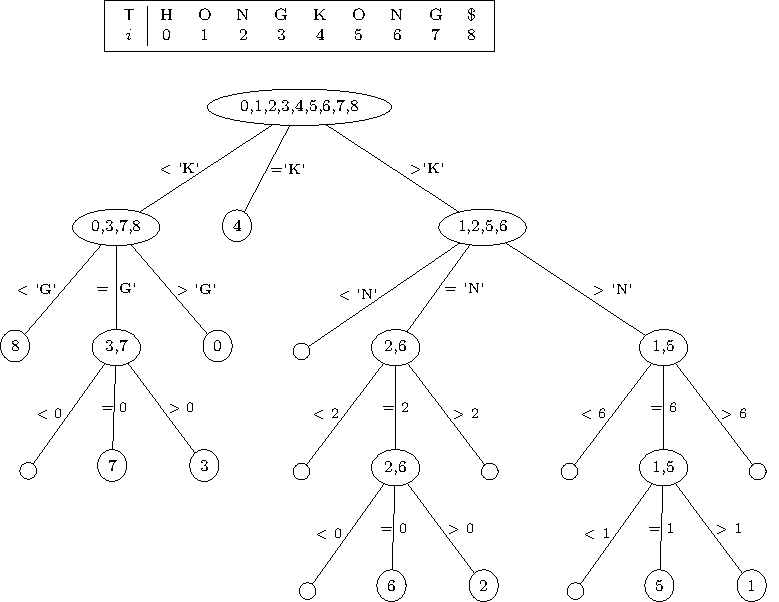
\includegraphics[scale=0.9]{kapitel/saca_algorithmen/qsufsort/Bilder/TerTree.pdf}
\caption{Der durch die ternäre Sortierung entstehende ternäre Baum anhand des Strings $\mathsf{T}=HONGKONG\$$.}
\label{terTree}
\end{figure}